\chapter{Introduction}
\label{ch:introduction}
	Forest covers approximately 30\% of the global land surface, while approximately 50\% of the global forest area is covered by tropical forest \citep{WWF2016}. Tropical forests covering the global land surface between 23$^\circ$ north (the tropic of Cancer) and 23$^\circ$ south (the tropic of Capricorn) around the equator as figure \ref{fig:tropicalzone} shows. This zone comprises several different forest types like tropical rain forest, tropical moist forest, tropical dry forest, and tropical mountain system forest. The distribution and extent of this forest types is affected by the following environmental properties: precipitation levels and seasonality, temperature profile, elevation, and soil characteristics. Rain forest account for approximately 60\% of the tropical forest cover and is characterized by warm and wet climate, while the average annual temperature is above 20 degrees and the precipitation ranges between 2500 and 4500 mm y$^{-1}$. The canopy is dense and dominated by trees with a height between 30 and 45 m. The required climate conditions are typically found between 10$^\circ$ north and 10$^\circ$ south. Tropical forest is a crucial part of our earth system as important factor for climate, water cycle, soil health, biodiversity storage, and source of natural goods for human subsistence. These forests are a major carbon sink and stimulate precipitation. Further, these forests house the largest diversity of species and a large amount of endemic species. However, this unique ecosystem is endangered by forest loss and transitions to other \ac{LULC} types \citep{WWF2016}.
	\begin{figure}[ht]
		\centering
		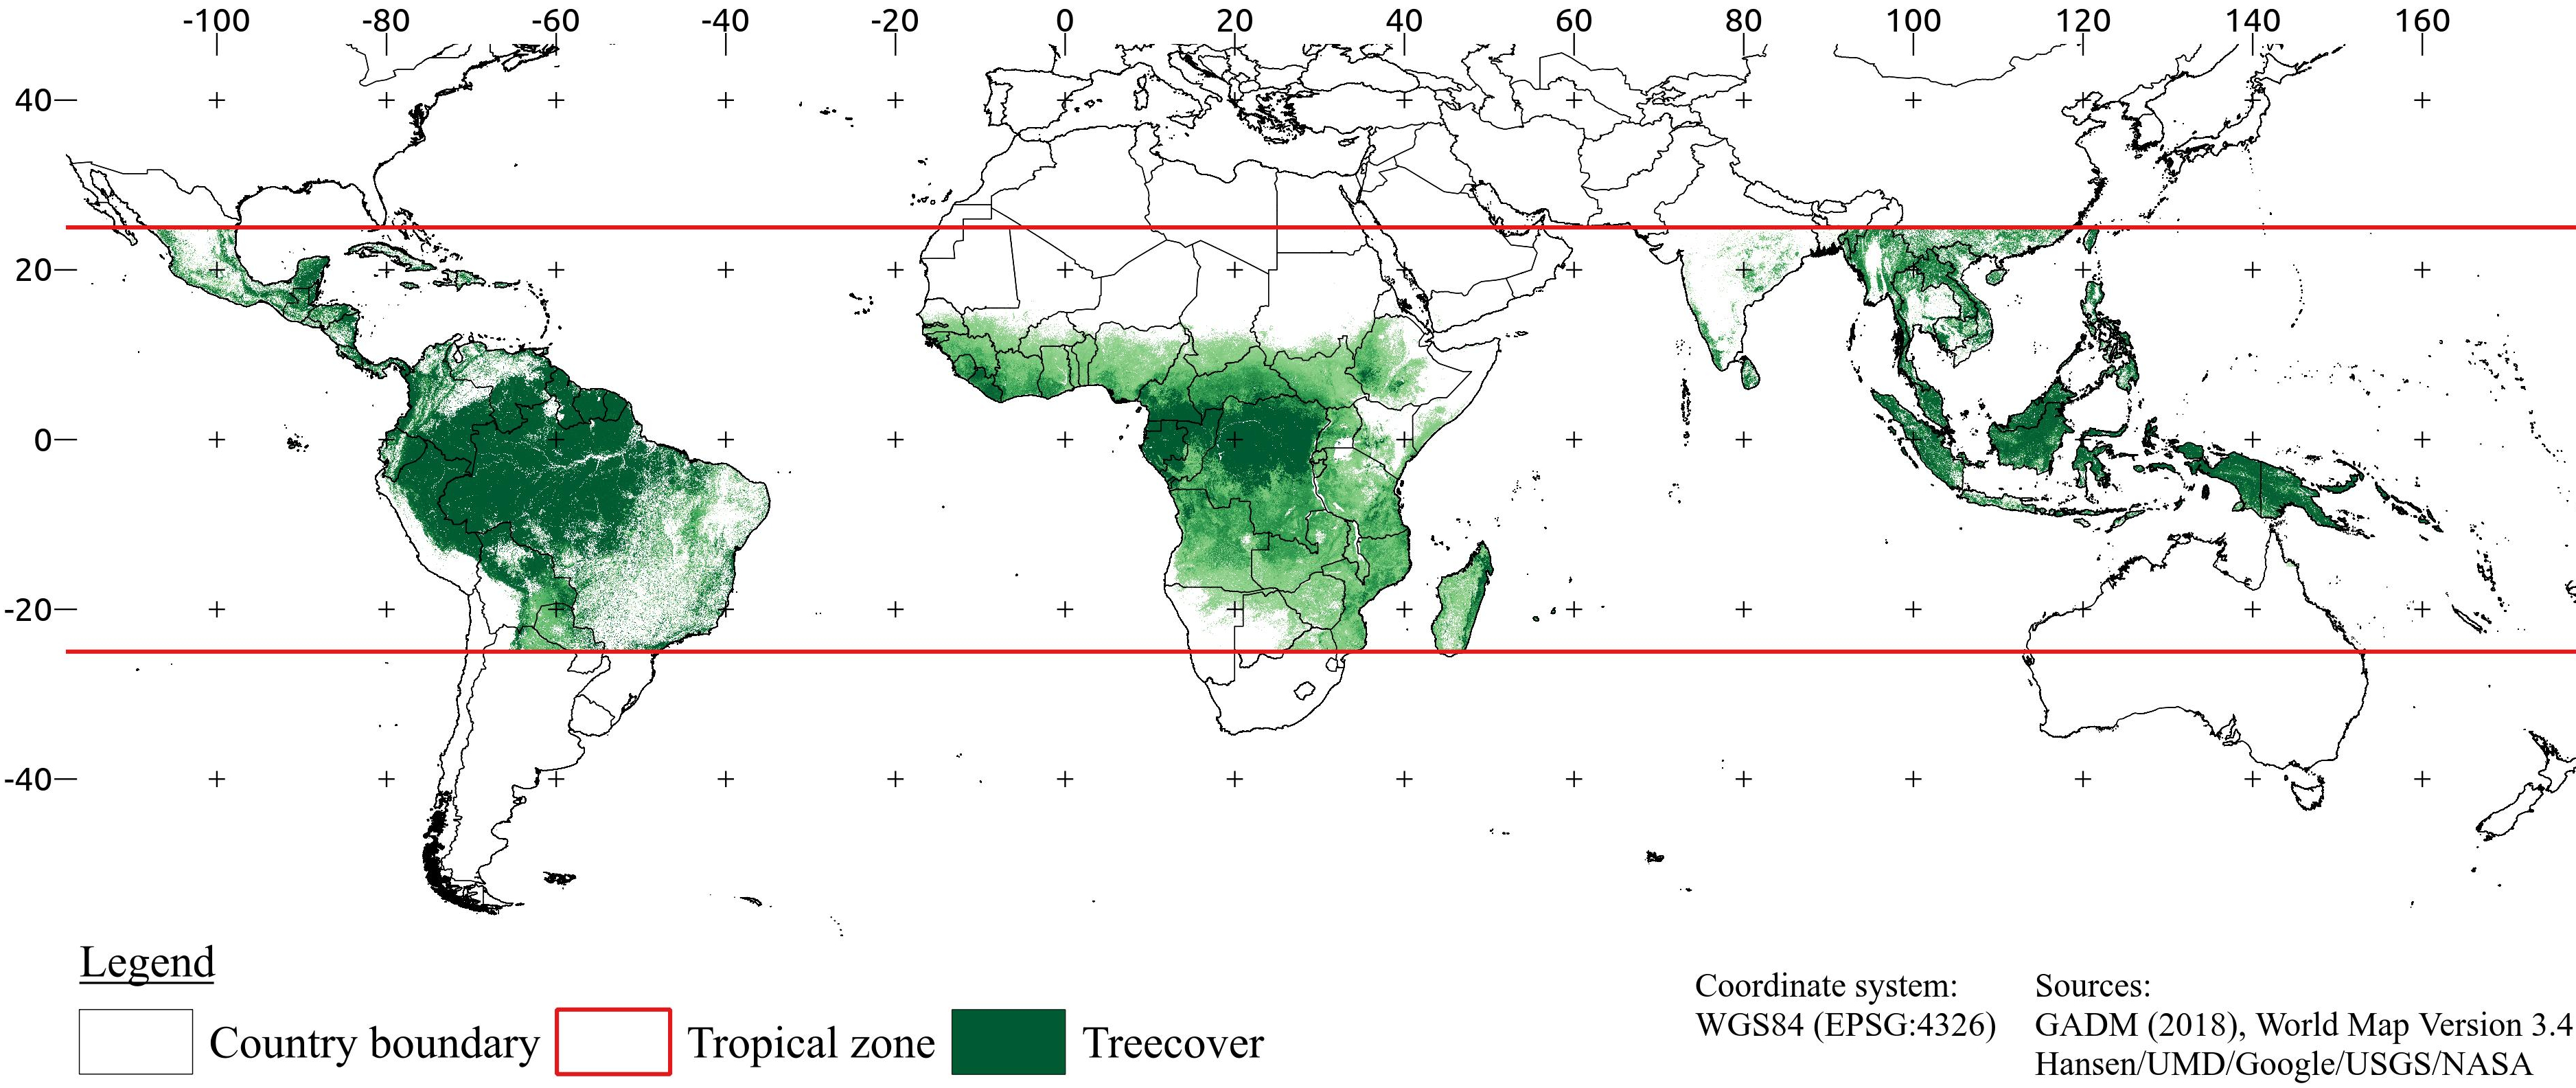
\includegraphics[scale=.97]{img/intro_overview_frameless}
		\caption[Tropical zone and forest]{\textbf{Tropical zone and forest}}
		\label{fig:tropicalzone}
	\end{figure}

	Since the 1990s approximately 3.1\% of the global forest area is lost, while approximately 35\% of the tree cover loss is within tropical forest cover \citep{FAO2016}. Between 1990 and 2015 all the top ten countries with the highest annul net loss of forest are located in the tropical zone \citep{FAO2010,FAO2016}. Forest loss or deforestation is defined as the removal of trees or forest stands from land surface which is subsequently converted to another \ac{LULC}. \citet{Geist2001} introduced the conceptual framework of proximate, underlying, and other causes of tropical deforestation to classify the drivers of forest cover change. Direct deforestation driver or proximate deforestation driver are anthropogenic actions that change forest to other \ac{LC} types. Proximate causes of deforestation are grouped into three different categories: agricultural expansion, wood extraction, and infrastructure expansion. Examples for deforestation driven by agriculture are the expansion of pastures, cropland, and tree crops as shown in figure \ref{fig:deforestationexamples}. Examples for wood extraction and infrastructure expansion would be the following categories: fuelwood extraction, charcoal production, transport infrastructure, and settlement expansion. Underlying causes are complex social, political, economic, technological, and cultural interactions, which underpin \acp{PDD}. The group of other causes for deforestation comprises land characteristics, biophysical drivers, and social trigger events. An example for the land characteristics is soil quality and topography of the landscape, which determines the shape of the deforestation. 

	Proximate drivers why bad, and good?
	Current state of science?

	Scientific studies of \acp{PDD} at a continental or regional range are common in science (e.g. \citet{Sy2015,Austin2019,Zalles2018,Meyfroidt2013,Caldas2013,Graesser2015,Ruf2014,Connette2016,Barima2016,Furumo2017,Vijay2018}). Whereas the frequency of global scaled studies on \acp{PDD} is lower (e.g. \citet{Curtis2018,Hosonuma2012,Geist2002,DeFries2010,Carter2018}). However, each of the beforehand mentioned studies tries to predict the \acp{PDD} by a varying methodology. Some studies relay on meta-analysis or auxiliary data from various sources for certain areas and an empirical approach to predict \acp{PDD} (e.g. \citet{Hosonuma2012,Geist2002,DeFries2010,Carter2018,Ruf2014}), while other studies uses sample-based methods combined with statistical models and visual interpretation of remotely sensed data from different sources (e.g. \citet{Sy2015,Austin2019,Curtis2018,Meyfroidt2013,Caldas2013}). Additionally, some studies relay only on remote sensing of the environment to predict the proximate causes of deforestation (e.g. \citet{Caldas2013,Zalles2018,Graesser2015,Connette2016,Barima2016}). On the fact that these studies need a vast amount of expert knowledge and in some cases repetition of time consuming processes they are hard repeatable on a annual basis. Further, the studies that estimate the \acp{PDD} spatially explicit are only in low resolution available \citep{Curtis2018,Caldas2013}. Additionally, all studies more or less present the proximate causes on deforestation already as aggregates of the three groups \citeauthor{Geist2001} suggest. Therefore, it is not possible to derive regional or continental differences between the patterns of cropland and pasture expansion.
	\begin{figure}[ht]
		\centering
		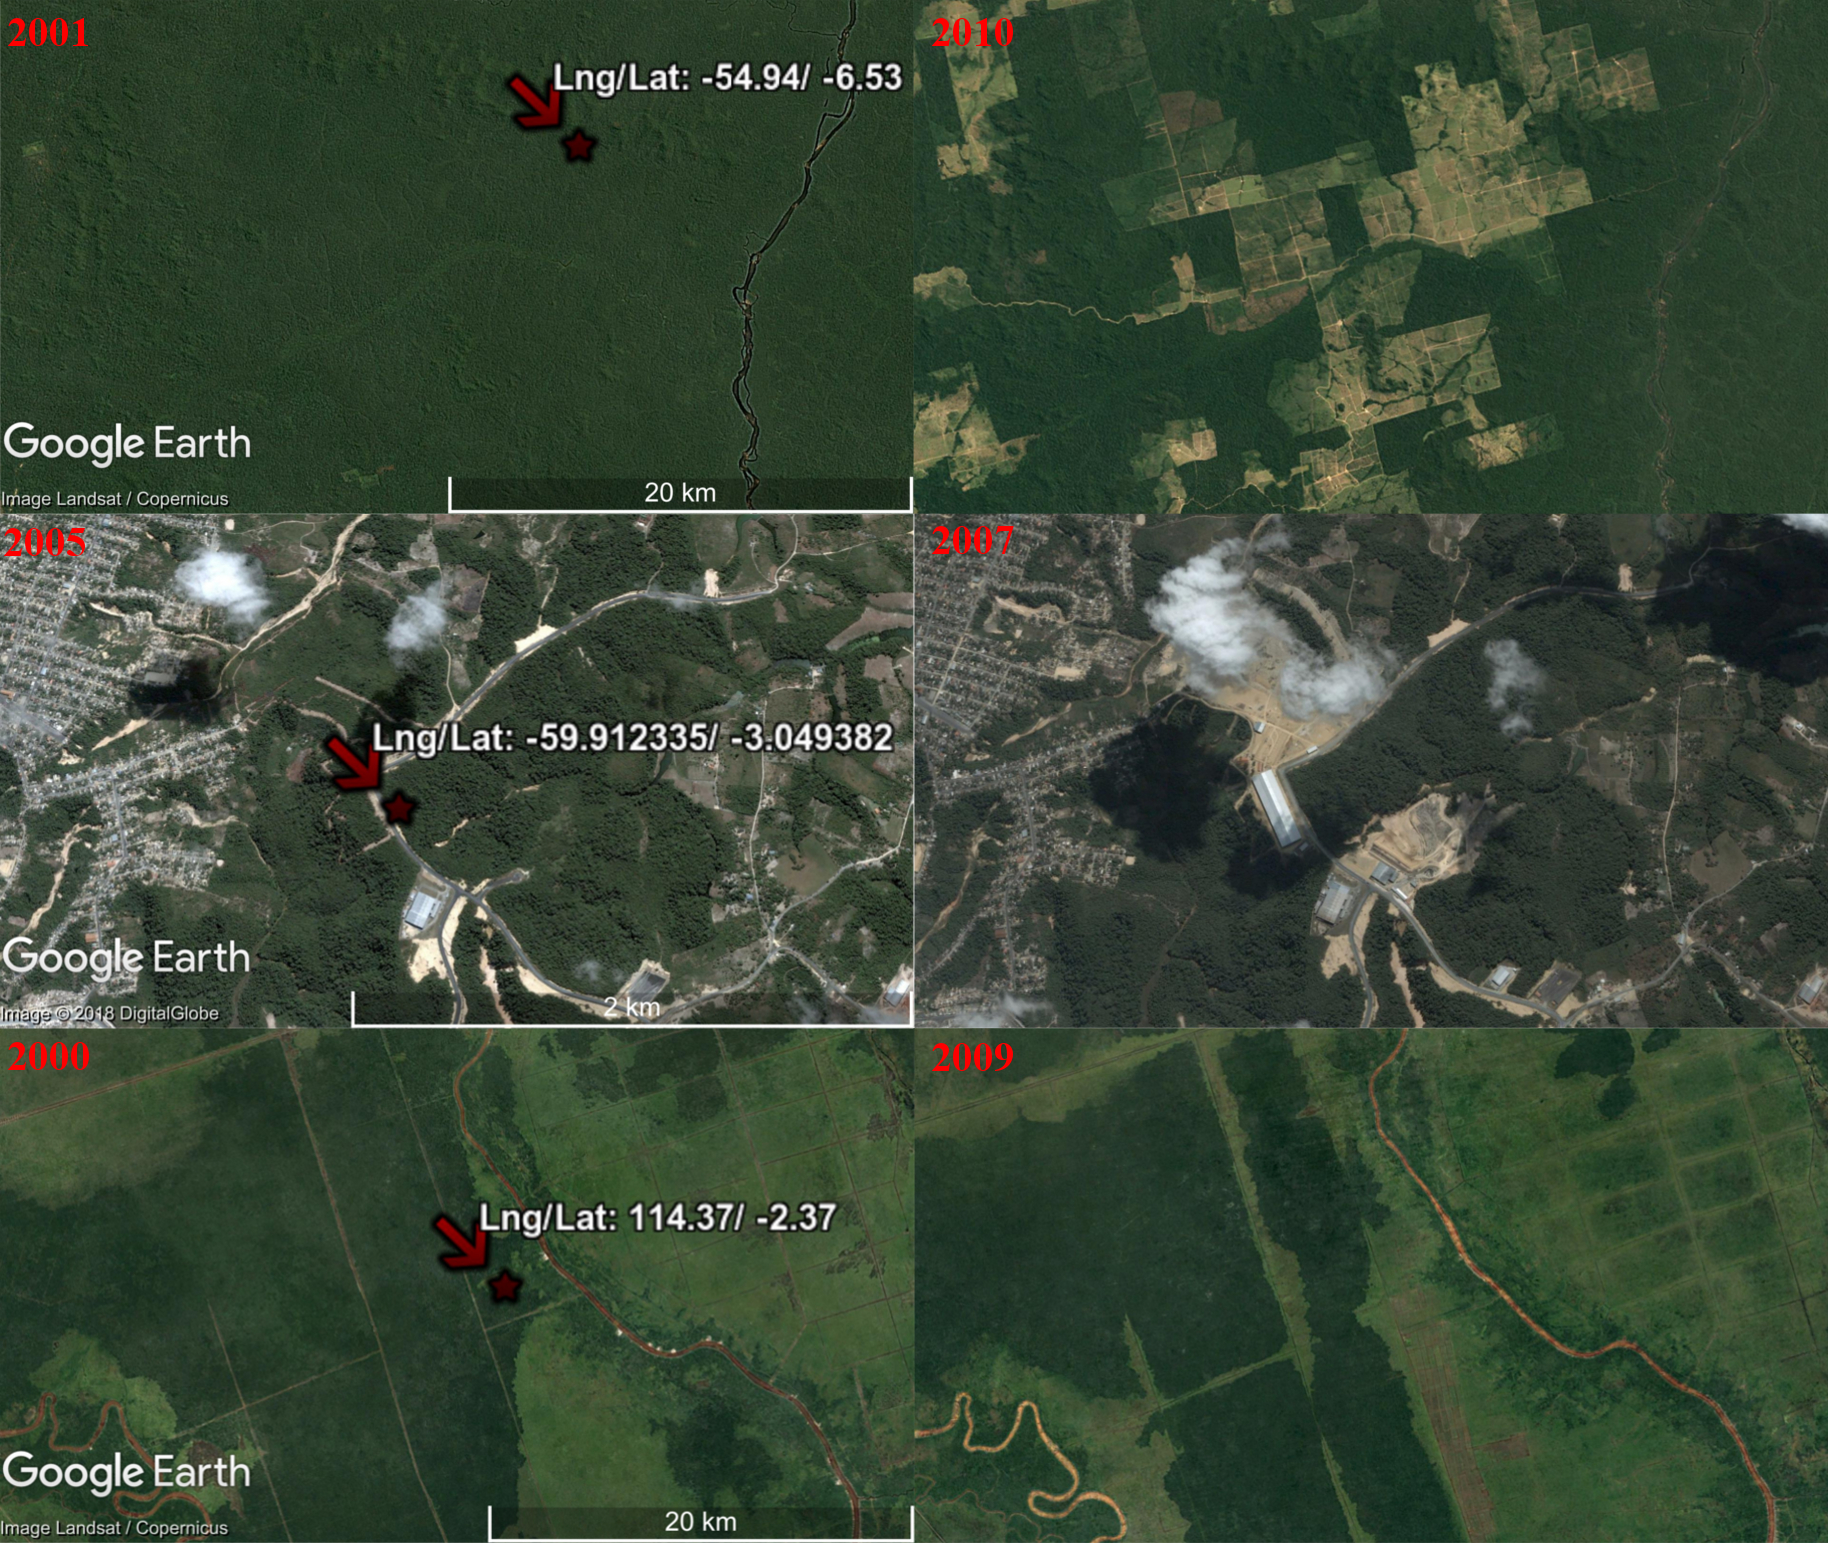
\includegraphics[scale=0.6]{img/deforestation_examples}
		\caption[Examples of proximate deforestation drivers]{\textbf{Examples of proximate deforestation drivers:} From top to bottom and left to right, pasture expansion in Brazilian rain forest, urban expansion in Brazil, and tree crop expansion in Indonesia.}
		\label{fig:deforestationexamples}
	\end{figure}

	Deforestation and its \acp{PDD} dynamic change the \ac{LC} type. These \ac{LC} changes are the second largest source of anthropogenic-induced \ac{GHG} emissions \citep{Don2010}. The removal of biomass and the changes of the \ac{SOC} are mainly responsible for this emissions. Why is important, What is state of science, What is missing

	Tropical forest ecosystems have a crucial impact on the well-being and subsistence of current and future generation out of humanity through the provision of regulatory, supporting, provisioning, and cultural services \citep{Costanza1997}. On the fact that deforestation and \ac{LC} changes lead to major changes in ecosystem services by altering the shape of forest biomes it is crucial to evaluate these impacts not only in terms of \ac{GHG} emissions but also for key ecosystem services as water, regulation, biodiversity etc. For the quantification of these ecosystem services a economic process is applied to assess the monetary value of each service per ecosystem. These \acp{ESV} can be a strong tool to determine the impact of certain management practices on ecosystem structures and raise the public awareness that ecosystems are scarce resources which could not be treated as free inexhaustible goods \citep{Groot2012}. The monetary valuation of ecosystems should be not understand as privatizing or commodifying them as tradeable goods for private markets \citep{Costanza2014,Song2018}. Further, the valuation of ecosystem services has fostered natural capital accounting and inclusion in national policies \citep{Song2018}. During the past decade scientific research fostered the development of several valuation approaches like direct market valuation, revealed preference, stated preference and benefit transfer \citep{Song2018}. Benefit transfer is the conceptually simplest approach to estimate the \ac{ESV}, but is widely used especially for estimates over large geographic regions \citep{Costanza1997,Song2018,Costanza2014}. This approach uses a constant unit value per hectare of ecosystem type and multiplies that value by the area of each type to obtain the aggregated total \citep{Costanza2014}. Remotely sensed land cover dataset are widely applied in the estimation \acp{ESV} to derive a global valuation of ecosystems by applying \ac{ESV} unit values \citep{Song2018}. The literature provides several studies on ecosystems and its monetary values. However, the by far most used global unit values for ecosystems are prepared by \citeauthor{Costanza2014}. This values are applied in several studies (e.g. \citet{Costanza2014,Song2018,Sannigrahi2018,Kreuter2001,Wang2006,Zhao2004}). \citet{Siikamaki2015} introduced recently global and regional \ac{ESV} unit values for forest ecosystems. These values are used by the World Bank in its wealth program on developing country-level indicators of sustainability \citep{Siikamaki2015}. Another well known datasets of \acp{ESV} is provided by \citet{Groot2012}. Till now several studies estimated \ac{ESV} dynamics at local or regional scales (e.g. \citet{Kreuter2001,Wang2006,Zhao2004}). Global-scale studies that estimate the monetary value of our planetary ecosystems and the losses by \ac{LC} change are relatively rare (e.g. \citet{Costanza1997,Costanza2014,Sannigrahi2018,Song2018}). The ecosystem estimates of this global studies ranging between 49.4-75.1 trillion dollar per year, while losses due to \ac{LC} change ranging between 1.21-20.2 trillion dollar per year, all values in 2007 Int'I\$ y$^{-1}$. The \ac{ESV} loss due to tropical deforestation ranges between 550.7 billion and 3.5 trillion dollar per year. These estimates are derived from \ac{LC} data at a coarse spatial resolution between 1 km and 300 m except the estimates of \citeauthor{Song2018}, that are derived from the \ac{GFC} dataset at spatial resolution of 30 m. However, the \ac{ESV} accounting of \citeauthor{Song2018} lacks of an importing filtering of the \ac{GFC} data and it does not consider \ac{ESV} dynamics from \ac{LC} change. Till now, to best of our knowledge no study accounted the \ac{ESV} dynamics in regards of \ac{ESV} loss, gain and balance exclusively for tropical forest loss and its \acp{PDD} by using high resolution data. 

	\section{Research objectives}
		Our research on mapping of the \acp{PDD} of tropical tree cover between 2000 and 2010 has the following objectives: 1) to determine spatial explicit the \acp{PDD} of tropical forest cover using 30 m resolution; 2) to derive forest transition patterns at regional, continental, and global scale; and 3) we wish to develop an approach, which is easy to reproduce and repeatable at certain time steps without to mush effort.

		For our research on gross \ac{GHG} emissions from tropical deforestation between 2000 and 2010 our objectives are: 1) to estimate the gross \ac{GHG} emissions through the removal of aboveground woody biomass; and 2) to estimate the gross \ac{GHG} emissions by \ac{SOC} change induced by \ac{LC} change.

		For our research on tropical \ac{ESV} dynamics between 2000 and 2010 our objectives are: 1) to estimate the loss in \ac{ESV} by anthropogenic deforestation of tropical forest cover; 2) to estimate the gain in \ac{ESV} by \ac{LC} transitions through \acp{PDD}; and 3) to account the balance as difference of gain and loss to determine the net loss or gain.